\chapter{Tecnologies}
\label{sec:tecnologies}

El programa que es vol desenvolupar durant el projecte ha d'utilitza les següents tecnologies: 

\begin{enumerate}
	\item{Test Driven Development com a metodologia de programació.}
	\item{Javascript com a llenguatge de programació.}
	\item{Node.js com a entorn d'execució del servidor. }
	\item{Websockets per a la comunicació entre el client i el servidor.}
	\item{HTML5,CSS i JQuery per a la capa de visualització del client.}
	\item{git com a programa de control de versions, utilitzant github per publicar el codi}
\end{enumerate}

\section{Perquè aquestes tecnologies?}

Abans de començar el projecte, quan en JM em va proposar de realitzar-lo em va dir que l'objectiu principal d'aquest projecte era provar, i a la vegada investigar el seu funcionament , noves tecnologies. Les que em va proposar són les següents: 
\begin{itemize}
	\item{Node.js}
	\item{Websockets}
	\item{HTML5, especialment l'objecte canvas}
\end{itemize}

Per la meva part desconexeia totalment l'existència de node.js i dels websockets. Tot i tenia petits coneixements sobre HTML5, sabia que aquest no eren molt extensos i que eren necessàri expandir-los.

El fet d'explorar noves tecnologies va ser molt motivador per mí, fins al punt de dir que ha estat una de les principals raons per decidir-m'he per aquest projecte i no per un altre. 

Per la meva part vaig decidir utilizar Test Driven Development com a metodologia de progamació perquè havia llegit alguna cosa sobre ell i em semblava bastant interesant. Tot i que normalment utilizo el diseny iteratiu, aquest treball em va semblar l'escusa perfecta per poder provar nous tipus de desenvolupament i així poder valorar quin d'ells és millor. 

Després d'explorar node.js vaig veure que el seu codi esta allotjat a github, i que la majoria dels móduls que corren sobre ell també. Així em va semblar convenient allotjar tot el codi del projecte al mateix lloc. Github utiliza git com software de control de versions

\section{Test Driven Development}

Test Driven Development o desenvolupament de software bastat en Testos es una metodologia de desenvolupament de software centrada en els jocs de proves. Aquesta metodologia utilitza el següent cicle de desenvolupament: 

\begin{figure}[htbp]
\centering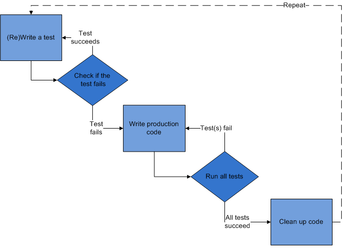
\includegraphics{test-driven-development.png}
\caption{Representació del cicle de desenvolupament basat amb TDD}
\label{fig:tdd}
\end{figure} 

\begin{enumerate}
    \item{Escriure un joc de prova.}
    \item{Executar tots els jocs de prova per comprovar que el nou test falla.}
    \item{Escriure el codi necesari per a que el joc de prova sigui favorable.}
    \item{Executar tots els jocs de provar per comprovar que tots els test son satisfactoris.}
    \item{Reestructurar el codi}
\end{enumerate}

A la figura \ref{fig:tdd} es pot veure un diagrama del cicle de desenvolupament basat en Test Driven Development.

Els pasos descrits anteriorment es duen a terme per a cada nova funcionalitat que es vol implementar. Aquesta metodologia té l'objectiu d'implementar petites funcionalitats que puguin ser provades de forma independent per un joc de prova, per tal de desprès juntar-les amb el conjunt de l'aplicació. 

%TODO: Fer una taula aqui?????
El Test Driven Deveolopment té les següents ventatges: 

\begin{enumerate}
    \item{Solidesa davant les fallades.}
    \item{Claretat dels requisits a implementar.}
    \item{Millora de la productivitat.}
\end{enumerate}

i els següents inconvenients: 

\begin{enumerate}
    \item{Difícil d'implementar en alguns casos: Interficies de client,bases de dades, programes depenents de la xarxa }
    \item{Dependencia de que els testos estiguin ben escrits. }
    
\end{enumerate}



\section{Javascript}

\section{Node.js}
%Tot i que node.js es un framwork bastant inusual, les primeres impresions ell van ser magnífiques. 
%Primer de tot utilitza codi Javascript per a crear servidors, quan tots els meus coneixements eren per executar codi Javascript en l'entorn de client. La segona cosa que em va sorprendre molt de node.js va ser que aquest sigui un entorn d'execució de programés asíncrons. 

\section{Websockets}

\section{HTML5}

\section{CSS}

\section{JQuery}

\section{Git i GitHub}

Git es un sistema de control de versions \footnote{\url{http://es.wikipedia.org/wiki/Control_de_versiones}} disenyat per Linus Trovalds, creador de Linux. Git té les següents característiques principals: 

\begin{description}
    \item[Suport per desenvolupament no lineal] Git està disenyat per tal de proporcionar una interficie rápida per a crear branques i mesclar-les.
    \item[Distribuït] Cada usuari té un repositori propi. Aquests respositoris poden ser fusionats amb respositoris d'altres usuaris.
    \item[Compatibilitat amb protocols existens] Els respositoris poden ser publicats mitjançant protocosl HTTP,FTP,Rsync i fins i tot un protocol propi.
    \item[Eficient per grans projectes] Git es ràpid i escalable. A més a més no es fa més lent a mesura que la història del projecte es fa gran, com pasa amb altres sistemes.
    \item[Portable] Funciona tan en sistemes Linux,Unix,MAC i Windows.
\end{description}

GitHub un servei de hosting de codi per a repositoris Git. A part d'allotjar el teu propi repositori ofereix altres serveis com poden ser Gist\footnote{\url{https://gist.github.com/}} (per a compartir petits trosos de codi), una wiki per projecte, allotjament de pàgines web i un petit gestió d'incidències molt flexible. A data 16/12/2011 compta amb 1,184,001 persones i allotja 3,448,813 repositoris.

GitHub ofereix il·limitats repositoris de forma gratuita sempre que el seu codi sigui públic. A més a més ofereix repositoris privats per un petit preu mensual. 


